% =====================================================================
%  Avoid Cartesian products: (R join S) join T  vs  (R x T) join S,
%  after [L14, s.25]
%  Compile:  pdflatex avoid-cartesian.tex   (inside this folder)
%  Output:   avoid-cartesian.pdf  -> 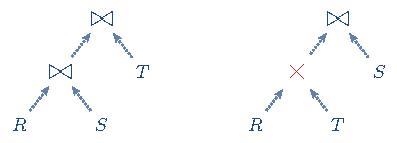
\includegraphics{avoid-cartesian}
% =====================================================================
\makeatletter\def\input@path{{../../theme/}}\makeatother   % shared palette
\documentclass[tikz,border=2pt,11pt]{standalone}
\usepackage[T1]{fontenc}
\usepackage[defaultsans]{lato}
\renewcommand{\familydefault}{\sfdefault}
\usepackage{amsmath,amssymb}
\usepackage{vinuni-palette}
\usetikzlibrary{arrows.meta}

\newcommand{\J}{\text{\Large$\bowtie$}}          % join node
\newcommand{\X}{\text{\Large$\times$}}           % cross-product node

\begin{document}
\begin{tikzpicture}[
    every node/.style={text=vinuNavy, font=\footnotesize},
    level distance=9mm, sibling distance=14mm,
    edge from parent/.style={draw=none},
    up/.style={-{Stealth[length=1.4mm]}, densely dotted, thick, vinuNavy!70}]

  % ---- (R join S) join T ------------------------------------------
  \node (a) {$\J$}
    child { node (a1) {$\J$} child { node (a11) {$R$} } child { node (a12) {$S$} } }
    child { node (a2) {$T$} };
  \foreach \c/\p in {a1/a, a2/a, a11/a1, a12/a1} \draw[up] (\c) -- (\p);

  % ---- (R x T) join S ---------------------------------------------
  \begin{scope}[xshift=40mm]
    \node (d) {$\J$}
      child { node (d1) {\textcolor{vinuRed}{$\X$}} child { node (d11) {$R$} } child { node (d12) {$T$} } }
      child { node (d2) {$S$} };
    \foreach \c/\p in {d1/d, d2/d, d11/d1, d12/d1} \draw[up] (\c) -- (\p);
  \end{scope}
\end{tikzpicture}
\end{document}
